See Fig. \ref{fig:3.8.5_qtwelve}.	
The velocity of rain and velocity of woman are
\begin{align}
\vec{v_r} &= \myvec{0\\-30}
\\
\vec{v_w} &= \myvec{-10\\0}
\end{align}
The relative velocity of rain w.r.t woman is given as
\begin{align}
\vec{v_{r_w}} &=\vec{v_r}- \vec{v_w}
\\
&=\myvec{10\\-30}
\end{align}
So the woman must hold the umbrella along the direction of $-\vec{v_{r_w}}$
Thus, the desired angle is 
\begin{align}
\theta={\tan}^{-1}\brak{\frac{10}{30}}
\end{align}
%
The following python code plots  Fig. \ref{fig:3.8.5_qtwelve}.
	\begin{lstlisting}
	./solutions/5/codes/lines/q12.py
	\end{lstlisting}
\begin{figure}[!ht]
	\centering
	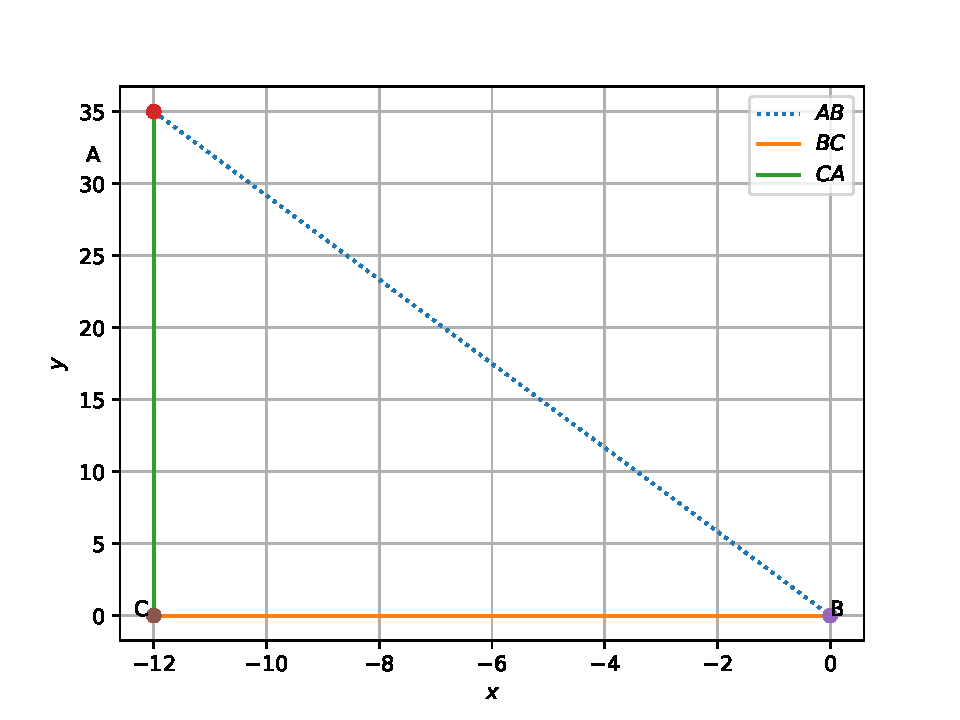
\includegraphics[width=\columnwidth]{./solutions/5/figs/lines/q12.eps}
	\caption{}
	\label{fig:3.8.5_qtwelve}	
	\end{figure}
	


